\documentclass[]{paper}
\usepackage{amsmath}
\usepackage{amssymb}
\usepackage{float}
\usepackage{tikz}
\usetikzlibrary{positioning,arrows.meta,fit,shapes.geometric}
\usepackage{pgfplots}
\pgfplotsset{compat=1.18}

\newcommand{\keep}{\textsc{keep}}
\newcommand{\edit}{\textsc{edit}}
\newcommand{\drop}{\textsc{drop}}
\newcommand{\run}[1]{\texttt{#1}}
\newcommand{\recallrule}{\cmidrule(lr){4-5}}

\begin{document}

\title{Status of the Synthetic Run}

\author[*]{Tatva Agarwal}
\author[*]{Vedant Kulkarni}
\author[*]{Bysani Vedavyas}
\author[*]{Venya Velmurugan}

\affiliation[]{IIIT Hyderabad}

\contribution[*]{Equal contribution; authors listed alphabetically.}

\abstract{
DiffusEdit repairs outdated sentences by masking stale tokens and infilling them with a frozen diffusion language model. This document records the full synthetic run: the pipeline, the data and its splits, the order of the runs and the checks between them, the metrics, the changes made during the run, every result, and the constraints on further work. On the synthetic test set the repair step with the heuristic ranking gains 0.038 ROUGE-L over leaving the sentence unchanged, and with a learned ranking of the same candidate pools it gains 0.054. A fully fine-tuned T5 editor gains 0.099 on the same sentences. The heuristic gain depends on two rules of the data generator and disappears when they are broken. The learned ranking keeps a gain of 0.019 when half of the new values are missing from the evidence.
}

\date{}
\correspondence{\email{vedant.kulkarni@students.iiit.ac.in}}

\maketitle{}


\section{Task and Terms}

An article is a list of sentences. Each sentence is labelled \keep{} (still correct), \edit{} (needs a change) or \drop{} (should be removed). The input is the outdated article and a few evidence passages. The output is the updated article.

DiffusEdit runs one forward pass of LLaDA-8B-Base over the evidence and the article. Small heads on the hidden states make the decisions. A linear sentence classifier assigns the labels. An attention staleness head scores each token of an \edit{} sentence as stale or not, and tokens above a threshold $\tau$ are masked. LLaDA infills each masked span at the lengths $0$, $\lceil n/2 \rceil$, $n$ and $n+2$, and the resulting candidate sentences are ranked by a reranker. The reranker score is $0.5\,\mathrm{PLL} + 0.5\,\mathrm{Ent}$, where PLL is the pseudo-log-likelihood of the sentence under LLaDA and Ent is the probability that the VitaminC verifier assigns to the best supporting evidence passage. A cascade detector then flags other sentences that a repair has made stale, such as an age after a birth date changes, and these sentences are repaired in a further round. LLaDA is frozen, and only the heads are trained.

The \emph{pool} of a sentence is the set of all candidates generated for it. \emph{Copy} is the unchanged source sentence. A \emph{gain} is a score minus the copy score.

\section{Pipeline}
\label{sec:pipeline}

\Cref{fig:pipeline} shows one round. One forward pass of LLaDA over the evidence followed by the article gives the hidden states of every token. Small heads on these states make every decision except the infilling.

\begin{figure}[t]
\centering
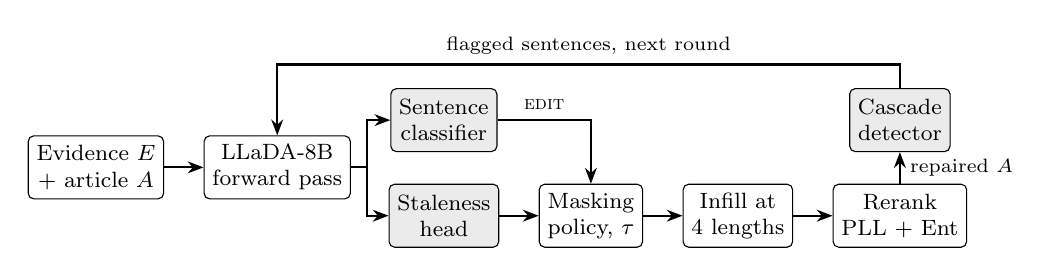
\begin{tikzpicture}[
  node distance=4mm and 5mm,
  box/.style={draw, rounded corners=2pt, align=center, font=\footnotesize, minimum height=8mm, inner sep=3pt},
  head/.style={box, fill=black!8},
  arr/.style={-{Stealth[length=2mm]}, thick}]
\node[box] (in) {Evidence $E$\\ + article $A$};
\node[box, right=of in] (llada) {LLaDA-8B\\ forward pass};
\node[head, right=of llada, yshift=6mm] (cls) {Sentence\\ classifier};
\node[head, below=of cls] (stale) {Staleness\\ head};
\node[box, right=of stale] (mask) {Masking\\ policy, $\tau$};
\node[box, right=of mask] (fill) {Infill at\\ 4 lengths};
\node[box, right=of fill] (rank) {Rerank\\ PLL + Ent};
\node[head, above=of rank] (casc) {Cascade\\ detector};
\draw[arr] (in) -- (llada);
\draw[arr] (llada.east) -- ++(2mm,0) |- (cls.west);
\draw[arr] (llada.east) -- ++(2mm,0) |- (stale.west);
\draw[arr] (cls.east) -| node[pos=0.25, above, font=\scriptsize] {\edit{}} (mask.north);
\draw[arr] (stale) -- (mask);
\draw[arr] (mask) -- (fill);
\draw[arr] (fill) -- (rank);
\draw[arr] (rank) -- node[right, font=\scriptsize] {repaired $A$} (casc);
\draw[arr] (casc.north) -- ++(0,3mm) -| node[pos=0.25, above, font=\scriptsize] {flagged sentences, next round} (llada.north);
\end{tikzpicture}

\caption{One round of DiffusEdit. Grey boxes are trained heads on the frozen LLaDA states. The cascade detector runs after the round and selects the sentences of the next round.}
\label{fig:pipeline}
\end{figure}

The sentence classifier is a linear layer on the mean state of a sentence at block 24 or 32 of LLaDA\@. The block with the higher val macro-F1 is used.

The staleness head scores each token of an \edit{} sentence. It compares the token's state with the evidence token states through learned attention with a null slot, so a token can attend to nothing when the evidence does not mention it. A linear head on the token state alone is the comparison.

The masking policy turns the token scores into spans. Tokens with a score of at least $\tau$ are masked. An empty mask falls back to the top fifth of the sentence, a mask over half of the sentence keeps its top half, and each span is widened to whole words. A token can be masked at most three times over all rounds.

Each span of $n$ masks is infilled at four lengths, $0$, $\lceil n/2 \rceil$, $n$ and $n+2$, so the repair can delete, shorten, keep or lengthen the span. Spans are decided left to right, and LLaDA decodes greedily in 8 steps. Each candidate sentence is scored by $0.5\,\mathrm{PLL} + 0.5\,\mathrm{Ent}$. PLL is the masked pseudo-log-likelihood of the sentence under LLaDA, and Ent is the probability that the VitaminC verifier \citep{schuster-etal-2021-vitaminc} assigns to the best evidence passage supporting the sentence.

The repair setting chosen on val (\cref{sec:protocol}) adds these rules to the base setting:
\begin{itemize}
\item an edit penalty, which subtracts 0.1 times the word edit distance between the candidate and the sentence before repair, so that a candidate is charged for every changed word \citep{chen-etal-2022-converge};
\item rejection of a candidate that adds a capitalised word or a number found in neither the evidence nor the sentence;
\item an evidence veto, which unmasks a span whose words all occur somewhere in the evidence;
\item a span cap, which leaves a sentence unrepaired when its mask has more than 2 spans;
\item evidence-copy candidates, which add 4 candidates per span that hold an evidence entity verbatim, chosen by their LLaDA likelihood in the span.
\end{itemize}

After a round, the cascade detector flags sentences outside the repaired set. The consequence head scores a pair of a repaired sentence and another sentence from their states before and after the repair. Staleness delta flags a sentence whose staleness scores rise after the round. Edited-as-evidence appends the repaired sentences to the evidence, so the next round reads them. A loop with no detector stops after one round. The loop runs at most 3 rounds.

A learned ranking replaces the score above in the runs marked \emph{learned ranking}. Every candidate is a whole sentence, so the logged pools can be ranked again without a model pass. A gradient-boosted tree classifier is fit on the pools of the val articles that chose v2 to predict whether a candidate has the best ROUGE-L of its pool, from the logged PLL, Ent and sampler confidence, the length rule, the word edit distance and ROUGE-L against the source, and the counts of capitalised words and numbers the candidate adds, split by whether the evidence holds them. The unchanged source joins every pool as one more candidate. The candidate with the highest predicted probability is the output.


\section{Data}
\label{sec:data}

The synthetic set is built from Wikipedia articles. One to three named entities of an \edit{} sentence are swapped for entities of the same spaCy type, and language model agents write evidence passages for the change. The set is used in reversed form. The real Wikipedia sentence is the outdated source, the swapped sentence is the gold update, and the evidence states the swapped values. In the forward direction, LLaDA recognised the swapped values as false from its pretraining, so a repair restored them without reading the evidence. Some kinds of swap were then undone to balance the share of stale words across word classes.

\begin{table}[H]
\caption{Splits of the reversed synthetic set. Supported articles have at least one \edit{} sentence whose new words all occur in the evidence or the source sentence. Linked articles hold a cascade sentence labelled by hand.}
\label{tab:data}
\centering
\footnotesize
\begin{tabular}{lrrr}
\toprule
 & Train & Val & Test \\
\midrule
Articles & 12,180 & 1,564 & 1,602 \\
\keep{} / \edit{} / \drop{} sentences & 27,061 / 12,360 / 3,062 & 3,472 / 1,575 / 414 & 3,500 / 1,684 / 428 \\
Evidence passages per article & 2.14 & 2.16 & 2.15 \\
Supported articles (\edit{} sentences) & & & 901 (1,670) \\
Linked articles (cascade sentences) & & & 220 (232) \\
\bottomrule
\end{tabular}
\end{table}

Of the 232 cascade sentences, 67 share an entity string with the direct edit and 165 do not. A detector that matches strings can only find the first group.

The generator guarantees that every new value of an \edit{} sentence occurs verbatim in the evidence and that no old value occurs anywhere in it. Update data taken from Wikipedia revisions, such as FRUIT, guarantees neither.

\section{Protocol}
\label{sec:protocol}

\subsection{Splits}

Heads are fit on train. Val sets early stopping, every threshold and every repair setting. Test is scored once per configuration. FRUIT val and test are not used. FRUIT train is used for one stress set only.

\subsection{Order of Runs}

\Cref{fig:order} shows the order of the runs and the two checks, called gates, that stop the queue when a stage does not improve on the stage before it.

\begin{figure}[t]
\centering
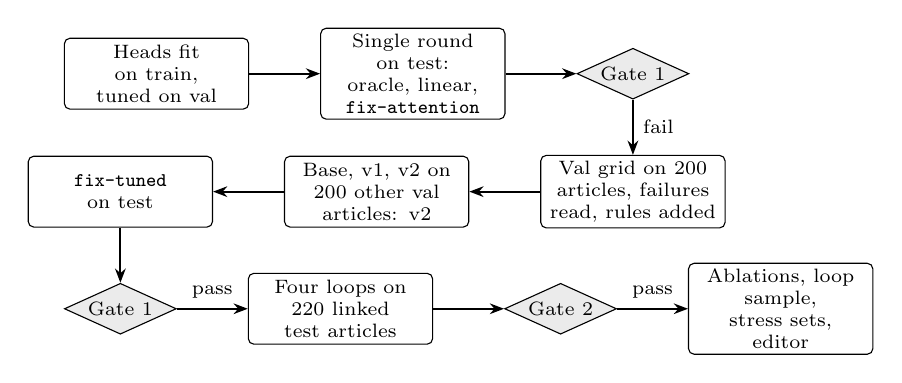
\begin{tikzpicture}[
  node distance=5mm and 9mm,
  box/.style={draw, rounded corners=2pt, align=center, font=\scriptsize, minimum height=9mm, text width=22mm, inner sep=2pt},
  gate/.style={draw, diamond, aspect=2.2, align=center, font=\scriptsize, inner sep=1pt, fill=black!8},
  arr/.style={-{Stealth[length=1.8mm]}, thick}]
\node[box] (heads) {Heads fit on train,\\ tuned on val};
\node[box, right=of heads] (fix) {Single round on test:\\ oracle, linear,\\ \run{fix-attention}};
\node[gate, right=of fix] (g1) {Gate 1};
\node[box, below=7mm of g1] (grid) {Val grid on 200\\ articles, failures\\ read, rules added};
\node[box, left=of grid] (fresh) {Base, v1, v2 on\\ 200 other val\\ articles: v2};
\node[box, left=of fresh] (tuned) {\run{fix-tuned}\\ on test};
\node[gate, below=7mm of tuned] (g1b) {Gate 1};
\node[box, right=of g1b] (loops) {Four loops on\\ 220 linked\\ test articles};
\node[gate, right=of loops] (g2) {Gate 2};
\node[box, right=of g2] (rest) {Ablations, loop\\ sample, stress sets,\\ editor};
\draw[arr] (heads) -- (fix);
\draw[arr] (fix) -- (g1);
\draw[arr] (g1) -- node[right, font=\scriptsize] {fail} (grid);
\draw[arr] (grid) -- (fresh);
\draw[arr] (fresh) -- (tuned);
\draw[arr] (tuned) -- (g1b);
\draw[arr] (g1b) -- node[above, font=\scriptsize] {pass} (loops);
\draw[arr] (loops) -- (g2);
\draw[arr] (g2) -- node[above, font=\scriptsize] {pass} (rest);
\end{tikzpicture}

\caption{Order of the runs. A failed gate stops every later stage. Gate 1 failed once, and the repair setting was then chosen again on val.}
\label{fig:order}
\end{figure}

The first single-round runs repair every supported test article once. They use oracle masks (the derived stale tokens), oracle masks without evidence, masks from the linear head and masks from the attention head. The run with attention-head masks is \run{fix-attention}.

Gate 1 requires \run{fix-attention} to gain at least 0.01 ROUGE-L over copying the source sentence. It gained 0.0091, so the queue stopped. The threshold $\tau$ was searched on 200 supported val articles, with and without the source span as an extra candidate. No setting gained more than 0.0097. The sentences of these runs were then read. They showed these failures:
\begin{itemize}
\item the reranker preferred the longest candidate, $n+2$, for 44\% of spans;
\item masks covered names and dates that were not stale;
\item for 15\% of sentences the gold update could not be produced from the input;
\item the model's prior outscored the evidence.
\end{itemize}
The five rules of \cref{sec:pipeline} were added in response. Base, v1 (the first four rules) and v2 (all five) were compared on 200 other supported val articles, because the first 200 had been read to design the rules. v2 was chosen. Its test run is \run{fix-tuned}, which passed gate 1.

Every loop run uses the predicted sentence labels and the attention-head masks with the v2 setting. The four main loops run on the 220 linked test articles. Gate 2 requires the consequence loop to raise cascade ROUGE-L over the single round and to lose no more than 0.01 UpdateROUGE-L. It passed.

The ablations, the stress sets and the editor baseline ran after gate 2.

\subsection{Samples}

The full test set does not fit the GPU budget for every ablation. The ablation sample holds 300 of the 901 supported test articles (557 \edit{} sentences). The loop sample holds 300 of the 1,602 test articles. Both samples were drawn with seed 42. Each comparison on a sample is made against its reference run restricted to the same articles.

\subsection{Stress Sets}

The stress sets break the guarantees of the generator. Both start from the 200 val articles on which v2 was chosen.
\begin{itemize}
\item In the missing-value set, for 183 of the 367 \edit{} sentences, every passage that holds a new value of the sentence is removed. 169 passages are removed, and 24 articles are left without evidence.
\item In the old-value set, one passage is added for each \edit{} sentence. The passage mentions the old values in another context and none of the new values. The passages were written by language model agents and checked by script. A passage fails the check if it omits an old value, holds a new value, copies seven consecutive words of the article, or has fewer than 10 or more than 80 words. All 367 passed.
\item The FRUIT set holds 200 FRUIT train articles with a stale \edit{} sentence.
\end{itemize}

\subsection{Seeds and Determinism}

Decoding is greedy, so a repair run gives the same output for the same head. The staleness head of every repair run was trained with seed 42 only. The confidence intervals therefore cover the sampling of test articles and not the training seed. The sentence classifier and the linear staleness head were trained with five seeds, and their seed spread is reported in \cref{tab:heads}.

\section{Metrics}
\label{sec:metrics}

\subsection{Sentence Repair}

The repair metrics are computed per \edit{} sentence against its gold update. Every run is scored on the same sentences, which are all gold \edit{} sentences of the articles it read, plus any other sentence it repaired. A sentence that the run left unrepaired is scored as its source sentence.
\begin{itemize}
\item \emph{ROUGE-L} is the ROUGE-L F1 of the output sentence. \emph{Copy} is the same score for the unchanged source sentence. The gain of a run is ROUGE-L minus copy.
\item \emph{Pool ROUGE-L} is the best ROUGE-L over all candidates the run generated. The difference from ROUGE-L is the loss due to the reranker.
\item \emph{Hit} is the share of sentences for which some candidate holds every new word of the gold update.
\item \emph{Repaired} is the share of sentences the run changed, and \emph{masked} the share of source characters it masked.
\item The \emph{supported} subset holds the sentences whose new words all occur in the evidence or the source sentence.
\end{itemize}

Copy scores 0.875 ROUGE-L on test, because an \edit{} sentence changes a few words and keeps the rest. A gain of 0.04 is therefore a large share of the 0.125 that copy leaves.

\subsection{Articles}

The article metrics compare the whole output article with the gold article. UpdateROUGE \citep{iv-etal-2022-fruit} is ROUGE between the output sentences that differ from the source and the gold sentences that differ from the source. An article with no changed output sentence scores 0. Entity precision and recall compare the entity mentions of the two sets of changed sentences. \emph{Unsupported} counts output mentions that occur in neither the source nor the evidence. \emph{Keep verbatim} is the share of gold \keep{} sentences that appear unchanged in the output.

Under UpdateROUGE a system that changes more sentences scores higher, because an unchanged sentence leaves the output side empty. The sentence metric scores an unchanged sentence as copy. The two metrics can therefore rank runs differently. On the ablation sample, removing the edit penalty raises UpdateROUGE-L by 0.12 and lowers sentence ROUGE-L by 0.008, because without the penalty more sentences are changed and more of the changes are wrong.

\subsection{Cascades}

\emph{Cascade ROUGE-L} is UpdateROUGE-L restricted to the cascade sentences. \emph{Cascade recall} is the share of cascade sentences that a detector flags in any round, split into sentences that share an entity string with the direct edit and sentences that do not.

\subsection{Detection}

The sentence classifier is scored by macro-F1 over the three labels. The staleness heads are scored by PR-AUC over the tokens of \edit{} sentences, since 11.3\% of these tokens are stale. The consequence head is scored by AUROC and F1 over sentence pairs.

\subsection{Tests}

Each comparison is paired over articles. Each metric is a ratio of sums over articles, so an article with more sentences carries more weight. The 95\% interval comes from a bootstrap that resamples whole articles, and the $p$-value from a permutation test that swaps the two systems within articles. The article metrics use 10,000 resamples and the sentence metrics 2,000. A Holm correction is applied over the tests of one comparison table.

\subsection{Values}

\emph{Exact match} is the share of output sentences equal to the gold update, ignoring case and spacing. Each synthetic edit has one correct answer, so exact match is defined for this data. \emph{New-value recall} is the share of gold new values that occur in the output as whole words, and \emph{old value kept} is the share of old values still in the output. Entity precision and recall, the count of output entities found in neither the source nor the evidence, and the share of \keep{} sentences left unchanged are also computed per article.

The value-level scores, the entity measures on the test sentences and new-entity precision were computed after the heuristic runs had finished, in a search for a measure on which DiffusEdit scores above the editor. They have not been used to choose any setting. A result found in this search is exploratory, and the full set of measures is reported here so that no measure is selected after the fact.


\section{Changes to the Pipeline}
\label{sec:changes}

\begin{itemize}
\item The synthetic set was reversed (\cref{sec:data}), because LLaDA recognised the swapped values without evidence in the forward direction.
\item LLaDA was loaded in bfloat16 without 4-bit quantization in every run, so that no result depends on quantization error.
\item The five repair rules of \cref{sec:pipeline} were added after gate 1 failed, and the setting was chosen on fresh val articles.
\item The sentence metric was changed to score the same sentence set for every run. It had scored only the sentences a run repaired, so a run that skipped hard sentences scored higher. Under the old metric v1 gained 0.031 on val, and under the new one 0.028. The earlier test runs repaired every sentence, so their numbers did not change.
\item A variable in the loop shadowed its timer, so every loop run failed on its first article. The variable was renamed, and the loops ran after a three-article check.
\item The spaCy entity file builder had overwritten the entity metric module. The builder was moved to its own module and the metric module restored.
\item The editor baseline ran out of GPU memory with batches of eight articles. It was trained with micro-batches of four articles, eight accumulation steps and gradient checkpointing, which keeps 32 articles per update.
\end{itemize}

\section{Results}
\label{sec:results}

\subsection{Heads}

\Cref{tab:heads} gives the test scores of the heads. The classifier and the linear staleness head lose most of their score when the evidence is removed from the input. The attention staleness head loses PR-AUC under both controls, so it reads the evidence.

\begin{table}[H]
\caption{Test scores of the heads. Five-seed values are mean $\pm$ standard deviation. The attention head and the consequence head were trained with seed 42 only.}
\label{tab:heads}
\centering
\footnotesize
\begin{tabular}{llc}
\toprule
Head & Measure & Test \\
\midrule
Sentence classifier, block 24 & Macro-F1, 5 seeds & $0.823 \pm 0.002$ \\
Sentence classifier, block 32 & Macro-F1, 5 seeds & $0.699 \pm 0.006$ \\
Sentence classifier, block 24, no evidence & Macro-F1, 5 seeds & $0.332 \pm 0.003$ \\
MiniLM baseline & Macro-F1, 5 seeds & $0.487 \pm 0.004$ \\
\midrule
Linear staleness head & PR-AUC, 5 seeds & $0.739 \pm 0.004$ \\
Linear staleness head, no evidence & PR-AUC, 5 seeds & $0.346 \pm 0.003$ \\
Attention staleness head & PR-AUC / AUROC & 0.831 / 0.966 \\
\quad evidence of another article & PR-AUC & 0.625 \\
\quad no evidence & PR-AUC & 0.718 \\
\midrule
Consequence head, 1,106 pairs & AUROC / F1 at $\tau_c = 0.35$ & 0.931 / 0.724 \\
\bottomrule
\end{tabular}
\end{table}

\subsection{Single-Round Repair}

\Cref{tab:repair} and \cref{fig:forest} give the single-round runs. Every gain except that of the linear-head masks is above zero. Oracle masks without evidence score below copy, so the gain of oracle masks comes from the evidence. \run{fix-tuned} gains 0.029 over \run{fix-attention} on the same sentences. Oracle masks with the v2 setting gain a further 0.023 over \run{fix-tuned} on the ablation sample. This difference is the gain that oracle masks would add to the v2 setting. The learned ranking of the same pools, \run{fix-rerank}, gains 0.016 $[0.013, 0.020]$ over \run{fix-tuned} on the 1,670 sentences, and 0.014 $[0.008, 0.019]$ over \run{fix-oracle-tuned} on the sample.

\begin{table}[H]
\caption{Single-round repair on test, sentence metrics. Runs above the rule cover the 1,670 \edit{} sentences of the 901 supported articles, and runs below it the 557 sentences of the ablation sample. Gain intervals are 95\% article bootstrap intervals.}
\label{tab:repair}
\centering
\footnotesize
\setlength{\tabcolsep}{4pt}
\begin{tabular}{llcccccc}
\toprule
Run & Masks, setting & ROUGE-L & Gain over copy & Pool & Hit & Repaired & Masked \\
\midrule
Copy & & 0.875 & & & & & \\
\run{fix-oracle} & oracle, base & 0.912 & $+0.037$ $[+0.032, +0.042]$ & 0.956 & 0.488 & 1.000 & 0.134 \\
\run{fix-oracle-noev} & oracle, base, no evidence & 0.854 & $-0.021$ $[-0.022, -0.019]$ & 0.916 & 0.014 & 1.000 & 0.134 \\
\run{fix-predicted} & linear head, base & 0.876 & $+0.001$ $[-0.004, +0.006]$ & 0.926 & 0.440 & 1.000 & 0.164 \\
\run{fix-attention} & attention head, base & 0.884 & $+0.009$ $[+0.005, +0.014]$ & 0.932 & 0.467 & 1.000 & 0.158 \\
\run{fix-tuned} & attention head, v2 & 0.912 & $+0.038$ $[+0.034, +0.043]$ & 0.952 & 0.628 & 0.875 & 0.117 \\
\run{fix-rerank} & attention head, v2, learned & \textbf{0.929} & $+0.054$ $[+0.049, +0.059]$ & 0.952 & 0.628 & 0.875 & 0.117 \\
\midrule
Copy & & 0.876 & & & & & \\
\run{fix-oracle} & oracle, base & 0.916 & $+0.039$ $[+0.032, +0.048]$ & & & & \\
\run{fix-tuned} & attention head, v2 & 0.918 & $+0.042$ $[+0.034, +0.050]$ & 0.952 & 0.633 & 0.865 & 0.110 \\
\run{fix-oracle-tuned} & oracle, v2 & 0.941 & $+0.064$ $[+0.055, +0.075]$ & 0.981 & 0.752 & 1.000 & 0.130 \\
\run{fix-oracle-rerank} & oracle, v2, learned & \textbf{0.955} & $+0.078$ $[+0.069, +0.089]$ & 0.981 & 0.752 & 1.000 & 0.130 \\
\bottomrule
\end{tabular}
\end{table}

\begin{figure}[t]
\centering
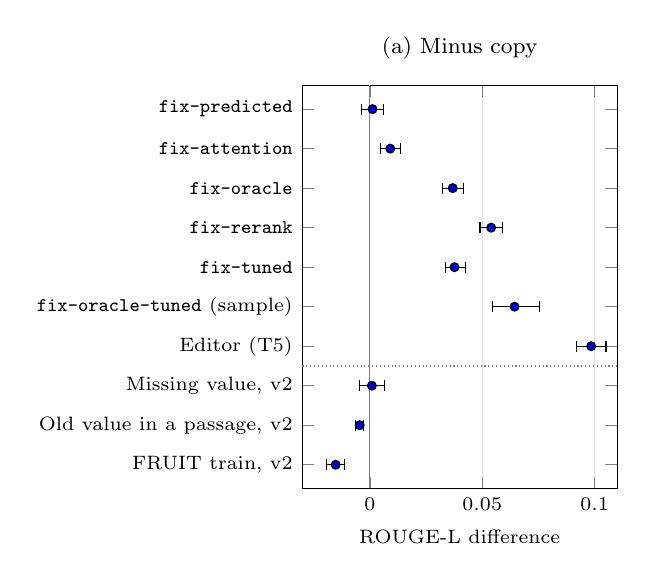
\begin{tikzpicture}
\begin{axis}[title={(a) Minus copy}, title style={font=\footnotesize}, width=0.46\linewidth, height=6.7cm,
  scale only axis=false, xmin=-0.03, xmax=0.11, ymin=-0.6, ymax=9.6,
  ytick={0,...,9}, yticklabels={{FRUIT train, v2},{Old value in a passage, v2},{Missing value, v2},{Editor (T5)},{\texttt{fix-oracle-tuned} (sample)},{\texttt{fix-tuned}},{\texttt{fix-rerank}},{\texttt{fix-oracle}},{\texttt{fix-attention}},{\texttt{fix-predicted}}}, yticklabel style={font=\scriptsize},
  xticklabel style={font=\scriptsize, /pgf/number format/fixed}, scaled x ticks=false,
  xlabel={ROUGE-L difference}, xlabel style={font=\scriptsize}, xmajorgrids, grid style={gray!25}]
\draw[gray] (axis cs:0,-0.6) -- (axis cs:0,9.6);
\draw[densely dotted, gray] (axis cs:-0.03,2.5) -- (axis cs:0.11,2.5);
\addplot+[only marks, mark=*, mark size=1.6pt, black, error bars/.cd, x dir=both, x explicit, error mark options={rotate=90, mark size=2pt}]
  coordinates {(-0.0152,0) += (0.0041,0) -= (0.0041,0) (-0.0045,1) += (0.0018,0) -= (0.0019,0) (0.0009,2) += (0.0056,0) -= (0.0055,0) (0.0985,3) += (0.0066,0) -= (0.0066,0) (0.0644,4) += (0.0110,0) -= (0.0099,0) (0.0377,5) += (0.0048,0) -= (0.0042,0) (0.0540,6) += (0.0051,0) -= (0.0050,0) (0.0369,7) += (0.0048,0) -= (0.0047,0) (0.0091,8) += (0.0047,0) -= (0.0043,0) (0.0012,9) += (0.0048,0) -= (0.0048,0)};
\end{axis}
\end{tikzpicture}\hfill
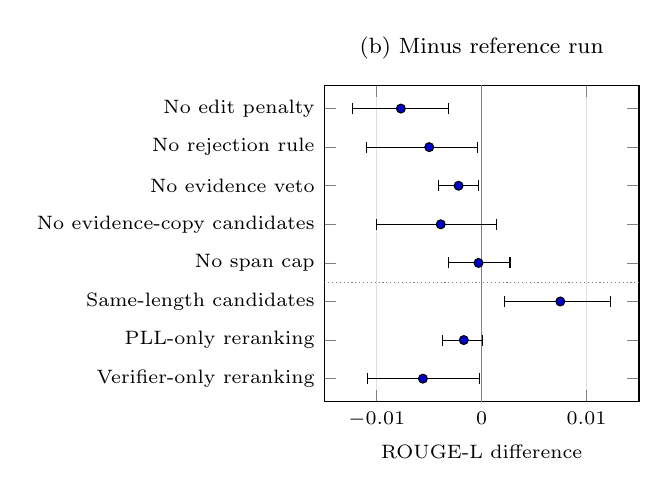
\begin{tikzpicture}
\begin{axis}[title={(b) Minus reference run}, title style={font=\footnotesize}, width=0.46\linewidth, height=5.60cm,
  scale only axis=false, xmin=-0.015, xmax=0.015, ymin=-0.6, ymax=7.6,
  ytick={0,...,7}, yticklabels={{Verifier-only reranking},{PLL-only reranking},{Same-length candidates},{No span cap},{No evidence-copy candidates},{No evidence veto},{No rejection rule},{No edit penalty}}, yticklabel style={font=\scriptsize},
  xticklabel style={font=\scriptsize, /pgf/number format/fixed}, scaled x ticks=false,
  xlabel={ROUGE-L difference}, xlabel style={font=\scriptsize}, xmajorgrids, grid style={gray!25}]
\draw[gray] (axis cs:0,-0.6) -- (axis cs:0,7.6);
\draw[densely dotted, gray] (axis cs:-0.015,2.5) -- (axis cs:0.015,2.5);
\addplot+[only marks, mark=*, mark size=1.6pt, black, error bars/.cd, x dir=both, x explicit, error mark options={rotate=90, mark size=2pt}]
  coordinates {(-0.0056,0) += (0.0054,0) -= (0.0053,0) (-0.0017,1) += (0.0018,0) -= (0.0020,0) (0.0075,2) += (0.0048,0) -= (0.0053,0) (-0.0003,3) += (0.0030,0) -= (0.0029,0) (-0.0039,4) += (0.0053,0) -= (0.0061,0) (-0.0022,5) += (0.0019,0) -= (0.0019,0) (-0.0050,6) += (0.0046,0) -= (0.0060,0) (-0.0077,7) += (0.0045,0) -= (0.0046,0)};
\end{axis}
\end{tikzpicture}

\caption{Sentence ROUGE-L differences with 95\% article bootstrap intervals. (a)~Each run minus copy. Test runs cover 1,670 sentences, ablation-sample runs 557, and stress sets 367 (408 for FRUIT). (b)~Each ablation minus its reference run on the 557 sentences of the ablation sample.}
\label{fig:forest}
\end{figure}

\subsection{Repair Ablations}

\Cref{tab:ablations} gives the ablations. With the v2 setting, removing the edit penalty, the rejection rule or the veto lowers ROUGE-L by an amount whose interval excludes zero. Removing the span cap or the evidence-copy candidates changes ROUGE-L by less than the interval width. With oracle masks and the base setting, same-length candidates score 0.0075 above the four-length set, PLL-only reranking is within noise of the combined score, and verifier-only reranking is 0.0056 lower.

\begin{table}[H]
\caption{Ablations on the 557 sentences of the ablation sample, sentence ROUGE-L minus the reference run. Top, attention-head masks against \run{fix-tuned} (0.918). Bottom, oracle masks against \run{fix-oracle} (0.916).}
\label{tab:ablations}
\centering
\footnotesize
\begin{tabular}{lccc}
\toprule
Change & Difference & 95\% interval & $p$ \\
\midrule
No edit penalty & $-0.0077$ & $[-0.0123, -0.0032]$ & 0.001 \\
No rejection of unsupported words & $-0.0050$ & $[-0.0110, -0.0004]$ & 0.028 \\
No evidence veto & $-0.0022$ & $[-0.0041, -0.0003]$ & 0.029 \\
No evidence-copy candidates & $-0.0039$ & $[-0.0100, +0.0014]$ & 0.153 \\
No span cap & $-0.0003$ & $[-0.0032, +0.0027]$ & 0.872 \\
\midrule
Same-length candidates only & $+0.0075$ & $[+0.0022, +0.0123]$ & 0.005 \\
PLL-only reranking & $-0.0017$ & $[-0.0037, +0.0001]$ & 0.067 \\
Verifier-only reranking & $-0.0056$ & $[-0.0109, -0.0002]$ & 0.035 \\
\bottomrule
\end{tabular}
\end{table}

\subsection{Learned Ranking}

The classifier was fit on the 367 pools of \run{repair-val2-v2}, which hold 2,890 candidates. Under five-fold cross-validation over the 200 val articles, with three fold assignments, the reranked pools score 0.933 ROUGE-L against 0.913 for the heuristic choice. Three tree sizes, a logistic regression, and extra training pools from the other val runs give gains between 0.012 and 0.020, and removing any one feature group changes the gain by at most 0.004. The configuration was fixed on val, and the test pools of \run{fix-tuned} were scored once with it.

On test the learned ranking changes the output of 780 of the 1,670 sentences. The heuristic ranking leaves 703 sentences equal to the source, including the 209 that the span cap leaves unrepaired, and chooses an evidence-copy candidate for 286 and a deletion for 26. The learned ranking leaves 279 unchanged and chooses an evidence copy for 519 and a deletion for 283. A deletion removes the stale value and scores above a wrong replacement under ROUGE-L, and the deletion choices carry 21\% of the test gain. A variant that never chooses a deletion gains 0.017 in the same cross-validation, with exact match 0.359 against 0.348, and has not been scored on test.

On the missing-value stress set, with the classifier fit on the clean pools outside a fold and applied to the stress pools inside it, the reranked pools gain 0.019 over copy where v2 gains 0.001, because the learned ranking leaves 42\% of the sentences unchanged where v2 leaves 30\%. On the old-value set the best candidate of the pool scores 0.883 against copy 0.882, since the veto unmasks nearly every span, and the reranked pools score 0.007 below copy against 0.005 for v2. That run used the val evidence for the features, because the added passages are only on the GPU host.


\subsection{Value-Level Scores}

\Cref{tab:values} scores the same test sentences by exact match and by the values. The editor corrects 89\% of the new values, against 40\% for \run{fix-tuned} and 50\% for \run{fix-rerank}. The v2 setting raises sentence ROUGE-L and exact match over \run{fix-attention} but lowers new-value recall and keeps more old values. v2 leaves 12.5\% of the sentences unchanged and masks 11.7\% of the characters, against none and 15.8\% for \run{fix-attention}. Fewer changes avoid damage to correct words and also leave more stale values in place.

\begin{table}[H]
\caption{Value-level scores on the 1,670 \edit{} sentences of the supported test articles, with 95\% article bootstrap intervals.}
\label{tab:values}
\centering
\footnotesize
\begin{tabular}{lccc}
\toprule
Run & Exact match & New-value recall & Old value kept \\
\midrule
Copy & 0.000 & 0.031 & 1.000 \\
\run{fix-attention} & 0.127 $[0.112, 0.142]$ & 0.435 $[0.412, 0.458]$ & 0.360 $[0.336, 0.386]$ \\
\run{fix-oracle} & 0.170 $[0.152, 0.188]$ & 0.446 $[0.422, 0.470]$ & 0.314 $[0.291, 0.338]$ \\
\run{fix-tuned} & 0.253 $[0.232, 0.274]$ & 0.395 $[0.373, 0.417]$ & 0.495 $[0.470, 0.521]$ \\
\run{fix-rerank} & 0.323 $[0.301, 0.345]$ & 0.499 $[0.476, 0.521]$ & 0.261 $[0.240, 0.281]$ \\
T5 editor & \textbf{0.767} $[0.747, 0.787]$ & \textbf{0.887} $[0.873, 0.902]$ & \textbf{0.100} $[0.086, 0.115]$ \\
\bottomrule
\end{tabular}
\end{table}

On the 557 sentences of the 300-article sample, \run{fix-oracle-tuned} reaches exact match 0.384 and new-value recall 0.502, so gold masks do not close the value gap to the editor either.

\subsection{Entity Measures}

The entity measures below cover the heuristic runs and the editor. They were not recomputed for \run{fix-rerank}, because the local environment lacks the entity extractor.

\Cref{tab:entities} gives the entity measures of the progress report on the same sentences. Mentions are spaCy entities and digit strings, extracted from each sentence alone. With $O$, $G$ and $S$ the mentions of the output, the gold update and the source, and $E$ those of the evidence, new-entity recall is $|O \cap (G \setminus S)| / |G \setminus S|$, new-entity precision is $|O \cap (G \setminus S)| / |O \setminus S|$, outdated kept is $|O \cap (S \setminus G)| / |S \setminus G|$, and fabricated is $|O \setminus (S \cup E)| / |O|$.

\begin{table}[H]
\caption{Entity measures on the 1,670 \edit{} sentences of the supported test articles, micro-averaged over sentences. Lower is better for the last two columns.}
\label{tab:entities}
\centering
\footnotesize
\setlength{\tabcolsep}{4pt}
\begin{tabular}{lcccccc}
\toprule
Run & Precision & Recall & New recall & New precision & Outdated kept & Fabricated \\
\midrule
Copy & 0.690 & 0.694 & 0.000 & & 1.000 & 0.000 \\
\run{fix-attention} & 0.738 & 0.759 & 0.407 & 0.416 & 0.304 & 0.169 \\
\run{fix-oracle} & 0.804 & 0.825 & 0.434 & 0.522 & 0.255 & 0.127 \\
\run{fix-tuned} & 0.795 & 0.789 & 0.366 & 0.667 & 0.472 & \textbf{0.048} \\
T5 editor & \textbf{0.940} & \textbf{0.943} & \textbf{0.855} & \textbf{0.901} & \textbf{0.100} & 0.079 \\
\bottomrule
\end{tabular}
\end{table}

The editor is better on every measure except fabricated entities. \run{fix-tuned} writes 323 fabricated mentions on the 1,670 sentences and the editor 533, which is 12.6 fewer per 100 sentences $[9.6, 15.4]$. On the 927 sentences that both runs change, the fabricated share is 0.086 for \run{fix-tuned} and 0.082 for the editor. The difference therefore comes from the sentences that \run{fix-tuned} leaves unchanged, and not from more faithful edits.

\subsection{Loss Breakdown}

\Cref{tab:pool} compares the candidate chosen by the reranker with the best candidate of the pool. The heuristic ranking loses 0.034 with attention-head masks and 0.040 with gold masks, and the learned ranking loses 0.022 and 0.026. The masks limit the pool. With the current masks, even a perfect reranker reaches 0.952, which is below the editor's 0.979. With gold masks and a perfect reranker, the pool reaches 0.981.

\begin{table}[H]
\caption{Chosen and best-of-pool sentence ROUGE-L on the 557 sentences of the 300-article sample.}
\label{tab:pool}
\centering
\footnotesize
\begin{tabular}{lcc}
\toprule
Masks & Chosen & Best of pool \\
\midrule
Attention head (\run{fix-tuned}) & 0.918 & 0.952 \\
Attention head, learned ranking (\run{fix-rerank}) & 0.930 & 0.952 \\
Gold (\run{fix-oracle-tuned}) & 0.941 & 0.981 \\
Gold, learned ranking (\run{fix-oracle-rerank}) & 0.955 & 0.981 \\
\bottomrule
\end{tabular}
\end{table}

\subsection{Stress Sets}

\Cref{tab:stress} gives the stress sets. On the missing-value set, v2 equals copy overall. On the 155 supported sentences, whose new words are still in the input, it gains 0.026, against 0.038 on the 317 supported sentences of the clean articles. The loss therefore comes mostly from the sentences whose new value is gone, which v2 still edits. On the old-value set, the masked share of v2 falls from 0.121 to 0.015, because the evidence veto unmasks every span whose words now occur in the added passage. v2 repairs 19\% of the sentences and scores 0.0045 below copy. On FRUIT both settings score below copy. Only 76 of the 408 FRUIT sentences have their new words in the input, so a perfect repair of those 76 would raise the FRUIT score by at most 0.027.

\begin{table}[H]
\caption{Stress sets, sentence ROUGE-L minus copy with 95\% article bootstrap intervals. The clean row is the same 200 val articles with their original evidence.}
\label{tab:stress}
\centering
\footnotesize
\begin{tabular}{lcccc}
\toprule
Set & Copy & Base & v2 & v2 repaired \\
\midrule
Clean val & 0.882 & $+0.008$ & $+0.031$ & 0.899 \\
Missing value & 0.882 & $-0.054$ $[-0.066, -0.043]$ & $+0.001$ $[-0.005, +0.007]$ & 0.703 \\
Old value in a passage & 0.882 & $-0.004$ $[-0.011, +0.004]$ & $-0.005$ $[-0.006, -0.003]$ & 0.193 \\
FRUIT train & 0.727 & $-0.057$ $[-0.064, -0.050]$ & $-0.015$ $[-0.019, -0.011]$ & 0.603 \\
\bottomrule
\end{tabular}
\end{table}

\subsection{Loops}

\Cref{tab:loops} gives the loops on the linked articles. Every detector raises cascade ROUGE-L over the single round. The consequence loop finds 79\% of the cascade sentences and edited-as-evidence 72\%, and the two loops do not differ in UpdateROUGE-L or cascade ROUGE-L within the intervals. The extra rounds change more sentences that should stay as they are, and keep verbatim falls from 0.929 to 0.898 for the consequence loop. Gold sentence labels raise UpdateROUGE-L by 0.044 over predicted labels.

\begin{table}[H]
\caption{Loops on the 220 linked test articles, article metrics. Cascade recall is over the 67 cascade sentences that share an entity string with the direct edit and the 165 that do not.}
\label{tab:loops}
\centering
\footnotesize
\setlength{\tabcolsep}{4pt}
\begin{tabular}{lcccccc}
\toprule
& Update & Cascade & \multicolumn{2}{c}{Cascade recall} & Entity & Keep \\
\recallrule
Detector & ROUGE-L & ROUGE-L & shared & unshared & precision & verbatim \\
\midrule
None (one round) & 0.436 & 0.210 & 0.000 & 0.000 & 0.866 & 0.929 \\
Staleness delta & 0.448 & 0.270 & 0.179 & 0.164 & 0.826 & 0.867 \\
Edited-as-evidence & \textbf{0.476} & 0.276 & 0.239 & 0.200 & 0.828 & 0.840 \\
Consequence & 0.470 & \textbf{0.296} & 0.358 & 0.352 & 0.847 & 0.898 \\
Consequence, gold labels & 0.514 & 0.339 & 0.030 & 0.115 & 0.890 & 1.000 \\
\bottomrule
\end{tabular}
\end{table}

The recall columns of \cref{tab:loops} count flags raised during the loop, after the repairs of earlier rounds. A separate detection test applies the gold rewrites of the direct edits and runs each detector once. Its recall is 0.793 for the consequence head, 0.720 for edited-as-evidence, 0.289 for string matching and 0.138 for staleness delta.

On the loop sample of 300 test articles, the consequence loop scores 0.014 UpdateROUGE-L above the single round, with an interval of $[0.000, 0.030]$. Without evidence, the consequence loop falls to 0.062 UpdateROUGE-L, from 0.490.

\subsection{Editor Baseline}

The editor is flan-t5-large fine-tuned on the 12,180 train articles to write the updated article from the outdated article and the evidence, in the style of EDIT5 \citep{iv-etal-2022-fruit}. It trained for 4 epochs and kept the checkpoint of epoch 3. On the 1,670 \edit{} sentences of the supported test articles it scores 0.973 ROUGE-L, a gain of 0.099 $[0.092, 0.105]$ over copy and 0.061 $[0.055, 0.067]$ over \run{fix-tuned}. On the loop sample it reaches UpdateROUGE-L 0.911 and cascade ROUGE-L 0.823, against 0.490 and 0.311 for the consequence loop. The editor was trained on the train split of the same generator, so it learns the generator's two guarantees from 12,180 examples. The stress sets were not run on the editor.

\begin{table}[H]
\caption{Cost on one A100. Total cost is training plus inference on the 1,602 test articles.}
\label{tab:cost}
\centering
\footnotesize
\begin{tabular}{lcc}
\toprule
 & DiffusEdit (\run{fix-tuned}) & T5 editor \\
\midrule
Trained parameters & 12.9M (heads only) & about 780M \\
Training GPU time & about 12 min & 64 min \\
Inference per article & 9.1 s & 0.35 s \\
Total GPU time & about 255 min & about 73 min \\
\bottomrule
\end{tabular}
\end{table}

\subsection{Results That Hold}

The sentence classifier on frozen LLaDA states reaches macro-F1 $0.823 \pm 0.002$ over five seeds, against $0.332$ when the evidence is removed from the input and $0.487$ for a MiniLM baseline. The attention staleness head reaches PR-AUC 0.831, and 0.625 when it reads the evidence of another article. The consequence detector flags 79\% of cascade sentences, against 29\% for string matching, and the consequence loop raises cascade ROUGE-L over the single round by 0.086 $[0.051, 0.124]$. The editor still scores higher on cascade sentences.

\section{Limitations}
\label{sec:limits}

The repair gain of v2 depends on the two guarantees of the generator. It is zero when half of the new values are missing from the evidence and negative when an old value occurs in a passage.

The repair rules were designed after the first test run failed gate 1, so the test set had been seen once before the setting was chosen. The setting itself was chosen on val articles that were not used to design the rules.

The stress sets that break the guarantees were built after the v2 setting was chosen, on the val articles that chose it. A method designed from the stress results would need a different kind of broken evidence for its final check.

Every repair and loop result comes from one staleness head trained with seed 42. The intervals cover the sampling of articles and not the variation across training seeds.

The editor baseline is fine-tuned on the full train split, while the DiffusEdit infiller is frozen and only its heads are trained. The two are compared on the same test sentences, but they differ in the amount of supervised update text they are trained on.

The ablations run on 300 of the 901 supported test articles, and the loop sample on 300 of 1,602 articles, so their intervals are wider than those of the full test runs.

\section{Constraints}

\begin{itemize}
\item The submission is due on 31 October at noon, as a formal LaTeX report with plots.
\item The GPU grant has INR 836.68 left, which is 9.9 A100 hours at INR 84.24 per hour. The instance is paused. It is resumed only to launch a job, it is paused as soon as no job runs, and each resume needs a new access token from the user.
\item LLaDA-8B-Base runs in full bfloat16 precision, never quantized and never the Instruct model.
\item FRUIT val and test are never used. FRUIT train may be used.
\item Test is scored once per configuration. Any new setting is chosen on val.
\item A method designed from the stress results needs a different kind of broken evidence for its final check, because the existing stress sets informed the design.
\item The user requires gains that hold beyond the generator's rules.
\end{itemize}

\section{Open Options}

\begin{itemize}
\item The no-deletion variant of the learned ranking on the test pools, which needs no GPU\@. It is a second test configuration and must be reported as such.
\item The T5 editor on the three stress sets, about 20 GPU minutes. On the missing-value set, v2 falls back to copy and rejects candidates that add names absent from the evidence, while the editor has no such rule. DiffusEdit may therefore score above the editor there, on ROUGE-L or on fabricated entities. This is the only comparison left in which DiffusEdit can come out ahead without a change to the method.
\item Both methods trained on 500 train articles and compared on the 300-article sample, about 1.5 to 2 GPU hours, to test whether the heads need less data than the editor.
\item Better masks, which raise the ceiling of the pool. Earlier changes to the head's loss and pooling moved its score by about 0.01, and a test run costs about 4 GPU hours.
\end{itemize}


\section{Files}

\begin{table}[H]
\centering
\footnotesize
\begin{tabular}{ll}
\toprule
Content & Location under \texttt{code/} \\
\midrule
Data splits & \texttt{datasets/synthetic/split/} \\
Pipeline code & \texttt{pipeline/infilling/}, \texttt{pipeline/staleness/}, \texttt{pipeline/cascading/} \\
Editor baseline & \texttt{pipeline/experiments/editor.py} \\
Stress set builder & \texttt{pipeline/experiments/stress.py} \\
Job queues & \texttt{pipeline/jobs/jl/} \\
Pulled results & \texttt{pipeline/outputs/jl/full/runs/} \\
Paired tests and figures & \texttt{pipeline/outputs/jl/full/analysis/} \\
Value-level scores & \texttt{pipeline/analysis/values.py} \\
Learned ranking & \texttt{pipeline/infilling/rerank.py} \\
Figures of the deep dive & \texttt{pipeline/analysis/evaluation.py} \\
Method walkthrough & \texttt{docs/internal/evaluation/evaluation.tex} (from the repository root) \\
\bottomrule
\end{tabular}
\end{table}

\bibliographystyle{plainnat}
\bibliography{../paper/paper}

\end{document}